\subsection{Фундаментальная система решений и общее решение нормальной линейной однородной системы уравнений (постоянные коэффициенты)}

Рассмотрим систему вида 
\begin{equation}
    \label{eq7:SLDE}
    \dot{\overrightarrow{x}} = A \overrightarrow{x} + \overrightarrow{f},
\end{equation} 
где $A = || a^i_j||$, $i,\,j = \overline{1, n}$ -- матрица системы, 
причём $a^i_j$ -- постоянные; 
$ \overrightarrow{f}(t) = 
  \begin{Vmatrix}
    f^1(t) \\
    \cdots    \\
    f^n(t)
  \end{Vmatrix}$ -- вектор-столбец неоднородной системы;
$\overrightarrow{x}(t) = 
\begin{Vmatrix}
  x^1(t) \\
  \cdots    \\
  x^n(t)
\end{Vmatrix}$ -- вектор-столбец искомых функций.  

Наряду с вышеприведённой записью также будем рассматривать запись вида: 
$$\frac{dx^i}{dt} = \sum\limits^n_{j=1}a^i_j x^j(t) + f^i, ~i = \overline{1, n}.$$

Основная идея решения систем дифференциальных уравнений вида \eqref{eq7:SLDE} 
состоит в том, что матрица системы рассматривается как матрица линейного преобразования 
линейного пространства $\overrightarrow{\mathbb{R}}^n$ (пространства, присоединённого к аффинному 
$\mathbb{R}^n$), заданная в исходном базисе (см. \hyperref[athenian_space]{определение афинного пространства} $\eqref{athenian_space}$).

Пусть $S = \begin{Vmatrix} \sigma_j^i \end{Vmatrix}$, $i,\,j = \overline{1, n}$ -- матрица перехода от исходного базиса $\begin{Vmatrix} \overrightarrow{e_1}, ..., \overrightarrow{e_n} \end{Vmatrix}$ к базису $\begin{Vmatrix} \overrightarrow{e'_1}, ..., \overrightarrow{e'_n} \end{Vmatrix}$. 
Эти соотношения связаны выражением $ \begin{Vmatrix} \overrightarrow{e'_1}, ..., \overrightarrow{e'_n} \end{Vmatrix}  = \begin{Vmatrix} \overrightarrow{e_1}, ..., \overrightarrow{e_n} \end{Vmatrix} \cdot S $ 
или $\overrightarrow{e'_i} = \sum\limits_{k = 1}^n \sigma_i^k \overrightarrow{e_k}$, а координаты векторов в новом и старом базисах связаны формулой $\overrightarrow{x} = S \overrightarrow{x'}$ или $x^i = \sum\limits_{m = 1}^n \sigma_m^i {x'}^m$.

Матрица перехода $S$ обратима, поэтому $\exists S^{-1} = \begin{Vmatrix} \tau_j^i \end{Vmatrix}$, $i,\,j = \overline{1, n}$, причём $SS^{-1} = S^{-1}S = E$, 
т.е. $\sum \limits_{k = 1}^n \tau_k^i \sigma_j^k = \delta_j^i$. Тогда $\overrightarrow{x'} = S^{-1}\overrightarrow{x}$.
Преобразуем исходную систему, умножив её справа на $S^{-1}$.

\[ S^{-1} \frac{d\overrightarrow{x}}{dt} = \frac{d}{dt} (S^{-1}\overrightarrow{x}) = S^{-1}A\overrightarrow{x} + S^{-1}\overrightarrow{f}.\]

Подставив $\overrightarrow x = S \overrightarrow{x'}$, получим $\frac{d\overrightarrow{x'}}{dt} = A' \overrightarrow{x'} + \overrightarrow{f'}$, где $\overrightarrow{f'}(t) = S^{-1}\overrightarrow{f}(t)$, 
а $A' = S^{-1}AS$ является матрицей преобразования $A$ в новом базисе. Уравнение имеет \textbf{ковариантный вид}, поэтому задачи свелись к нахождению базиса, в котором система имела бы наиболее простой вид.

Пусть $A$ -- матрица системы \eqref{eq7:SLDE} является матрицей линейного преобразования линейного пространства $\overrightarrow{\mathbb{R}}^n$, 
т.е. $\forall \overrightarrow{x} \in \overrightarrow{\mathbb{R}}^n \mapsto A\overrightarrow{x} = \overrightarrow{y} \in \overrightarrow{\mathbb{R}}^n$, тогда $A = \begin{Vmatrix} A\overrightarrow{e_1}, ..., A\overrightarrow{e_n} \end{Vmatrix}$, 
т.е столбцы матрицы $A$ являются компонентами образов базисных векторов.

\begin{definition}
    Подпространство $L \subset \overrightarrow{\mathbb{R}}^n$ называется \textbf{инвариантным} подпространством относительно преобразования $A$, если $\forall \overrightarrow{x} \in L \mapsto A \overrightarrow{x} \in L$.
\end{definition}

Пусть $\overrightarrow{e}_1, ..., \overrightarrow{e}_s, \overrightarrow{e}_{s+1}, ..., \overrightarrow{e}_n$ -- базис в $\overrightarrow{\mathbb{R}}^n$, а $\overrightarrow{e}_1, ..., \overrightarrow{e}_s$ -- базис в $L$. \\
Тогда $\forall i = \overline{1, s} \mapsto A\overrightarrow{e_i} = \sum\limits_{k=1}^s \gamma_i^k \overrightarrow{e_k}$ и матрица $A$ в этом базисе будет иметь вид:

\[ A = \begin{Vmatrix} A_1 & A_2 \\ O & A_3 \end{Vmatrix}, \text{ где } A_1 = \begin{Vmatrix} \gamma_1^1 & \cdots & \gamma_s^1 \\ \vdots & & \vdots \\ \gamma_1^s &\cdots & \gamma_s^s\ \end{Vmatrix}, ~O \text{ - нулевая матрица размером } (n - s) \times s. \]

Если $\overrightarrow{\mathbb{R}}^n = L^1 \oplus ... \oplus L^k$ и $L^i, ~i = \overline{1, k}$ -- инвариантные подпространства, то в базисе, который является базисом-объединения всех базисов инвариантных подпространств, прямая сумма которых равна $\overrightarrow{\mathbb{R}}^n$, матрица будет иметь вид:
\[A = \begin{Vmatrix} A_1 & O & \cdots & O \\ O & A_2 & \cdots & O \\ \cdots & \cdots & \cdots & \cdots \\ O & O &\cdots & A_k \end{Vmatrix}, \]
где $A_i, ~i = \overline{1, k}$ -- квадратная матрица размерами $l_i < n$, которая является сужением матрицы преобразования $A$ на инвариантное подпространство $L_i$.

В таком случае искомую вектор-функцию можно переписать в виде: 
\[ \overrightarrow{x}(t) = \begin{Vmatrix} x^1 \\ \cdots \\ x^{l_1} \\ \cdots \\ x^{l_1 + ... + l_{i-1} + 1} \\ x^{l_1 + ... + l_{i}} \\ \cdots \\ x^{l_1 + .. l_k + 1} \\ \cdots \\ x^n \end{Vmatrix}\]

\[\text{Обозначим через } X_i = \begin{Vmatrix} x^{l_1 + ... + l_{i-1} + 1} \\ \cdots \\ x^{l_1 + .. + l_{i-1} + l_{i}}\end{Vmatrix}. \]

Тогда система \eqref{eq7:SLDE} распадается на $k$ систем, порядок которых $l_i < n$: \\
$\dot{\overrightarrow{X_i}} = A_i \overrightarrow{X_i} + \overrightarrow{f_i}(t), ~i =\overline{1, k}$.

Для приведения матрицы линейного преобразования к клеточно-диагональному виду нужно найти собственные векторы линейного преобразования. 
Вектор $\overrightarrow{x} \neq 0$ называется собственным вектором линейного преобразования, матрица которого равна $A$, если $A\overrightarrow{x} = \lambda \overrightarrow{x}$. 
Пусть $A = \begin{Vmatrix} a_j^i \end{Vmatrix}, ~i,\,j = \overline{1, n}$, а $\begin{Vmatrix} x^1 \\ \cdots \\ x^n \end{Vmatrix}$ -- компоненты собственного вектора.
Тогда компоненты собственного вектора должны удовлетворять системе однородных линенейных уравнений вида $|| A - \lambda E|| \overrightarrow{x} = 0$. 
Чтобы эта система имела ненулевое решение необходимо, чтобы $\det || A - \lambda E|| = P_n(\lambda) = (-1)^n \lambda^n + (-1)^{n-1} \Tr A + ... + \det A = 0$. \\
$P_n(\lambda)$ -- характерестический многочлен матрицы $A$. 

\subsubsection*{Случай простых корней характеристического многочлена}
Рассмотрим однородную систему с постоянными коэффициентами
\begin{equation}
  \dot{\overrightarrow{x}} = A \overrightarrow{x} \label{eq:ODN}
\end{equation} 
Задача состоит в том, чтобы найти вектор функции $\overrightarrow{x}_1, \, \dots, \, \overrightarrow{x}_n$, которые будут образовывать ФСР нашей системы. Для удобства выделим несколько различных случаев.

\subsubsection*{Корни характеристического многочлена $\lambda_1, \dots, \lambda_n$ простые и действительные}

Таким $\lambda_1, \dots, \lambda_n$ соответствуют собственные векторы $\overrightarrow{h}_1, \dots, \overrightarrow{h}_n$ ($A \overrightarrow{h}_i = \lambda_i \overrightarrow{h}_i$)
Можно показать, что собственные вектора, соответствующие разным собственным значениям, линейно независимы, 
поэтому существует базис из собственных векторов $\overrightarrow{h}_1, \dots, \overrightarrow{h}_n$, в котором матрица $A$ имеет вид: 
$A' = \begin{Vmatrix} \lambda_1 & 0 & \ldots & \\ 0 & \lambda_2 & \ldots \\  \vdots& \vdots & \ddots &  0 \\ & & 0 & \lambda_n \end{Vmatrix}$.
Тогда система \eqref{eq:ODN} будет иметь следующий вид: 
\[ \begin{cases}
    \cfrac{d \overrightarrow{x\,}^1}{dt} = \lambda_1 \overrightarrow{x \,}^1 \\
    \cdots \\
    \cfrac{d \overrightarrow{x \,}^n}{dt} = \lambda_n \overrightarrow{x \,}^n
\end{cases} \Longrightarrow \]
вектор-функции $\varphi_1 = \begin{Vmatrix*} 1 \\ 0 \\ \vdots \\ 0 \end{Vmatrix*} e^{\lambda_1 t}$, ..., 
$\varphi_n = \begin{Vmatrix*} 0 \\ 0 \\ \vdots \\ 1 \end{Vmatrix*} e^{\lambda_n t}$ 
образует ФСР этой системы, т.к. являются линейно независимыми решениями.
Матрица перехода в этом случае $S = \begin{Vmatrix*} \overrightarrow{h}_1,  ...,  \overrightarrow{h}_n \end{Vmatrix*}$. 
Тогда получим, что
\begin{equation}
  \overrightarrow{x}_1 = \overrightarrow{h}_1 e^{\lambda_1 t}, ..., \overrightarrow{x}_n = \overrightarrow{h}_n e^{\lambda_n t} \label{eq7:FSR}
\end{equation} является ФСР \eqref{eq:ODN}, т.к. $\overrightarrow{x}_i, \,i= \overline{1, n}$ из \eqref{eq7:FSR} являются решениями \eqref{eq:ODN}, 
линейная независимость вектор-функций $\overrightarrow{x}_1, ..., \overrightarrow{x}_n$ следует из того, что вронскиан \eqref{eq7:FSR} при $t=0$ является $det S \neq 0$ (следует из свойств вронскиана, см. $\eqref{wr_properties}$).
Тогда любое решение \eqref{eq:ODN} представимо в виде
\begin{equation}
  \overrightarrow{x} = C_1 \overrightarrow{h}_1 e^{\lambda_1 t} + ... + C_n \overrightarrow{h}_n e^{\lambda_n t}.
\end{equation}

\begin{lemma}
  Система функций $e^{\lambda_1t}, ..., e^{\lambda_n t}$, где все $\lambda_i$ -- разные, является линейно независимой.  
\end{lemma}
\begin{proof}
  Составим линейную комбинацию, равную нулю: $C_1 e^{\lambda_1 t} + ... + C_n e^{\lambda_n t} = 0$ -- продифференцируем $(n-1)$ раз и 
  запишем получившуюся систему для поиска $C_1, ..., C_n$

  \[
  \begin{cases}
    C_1 e^{\lambda_1 t} + ... + C_n e^{\lambda_n t} = 0 \\
    \lambda_1 C_1 e^{\lambda_1 t} + ... + \lambda_n C_n e^{\lambda_n t} = 0 \\
    \cdots \\
    \lambda_1^{n-1} C_1 e^{\lambda_1 t} + ... + \lambda_n^{n-1} C_n e^{\lambda_n t} = 0
  \end{cases} 
  \]
  Система является однородной, поэтому имеет тривиальное решение, но единственное ли оно? 

  \[ \Delta = \begin{vmatrix*}
    e^{\lambda_1 t} & \cdots & e^{\lambda_n t} \\
    \lambda_1 e^{\lambda_1 t} & \cdots & \lambda_n e^{\lambda_n t} \\
    \vdots &  & \vdots \\ 
    \lambda_1^{n-1} e^{\lambda_1 t} & \cdots & \lambda_n^{n-1} e^{\lambda_n t} \\
  \end{vmatrix*} = e^{\lambda_1 t + ... + \lambda_n t} \begin{vmatrix*}
    1 & \cdots & 1 \\
    \lambda_1  & \cdots & \lambda_n  \\
    \vdots &  & \vdots \\ 
    \lambda_1^{n-1}  & \cdots & \lambda_n^{n-1} \\
  \end{vmatrix*} = e^{\lambda_1 t + ... + \lambda_n t} \prod \limits_{1 \leq j < i \geq n} (\lambda_i - \lambda_j) \neq 0
  \]

  Полученный определитель это определитель Вандермонда, который равен нулю только если какая-то пара $\lambda_i, \lambda_j$ совпадёт. 
  Значит, определитель не равен нулю по условию $\Rightarrow$ система имеет только тривиальное решение по теореме Крамера $\Rightarrow$ система линейно независима.
\end{proof}

\begin{lemma}
Система $\overrightarrow{\varphi}_1 = \overrightarrow{h}_1 e^{\lambda_1 t}, ..., \overrightarrow{\varphi}_n = \overrightarrow{h}_n e^{\lambda_n t}$ является ФСР. 
\end{lemma}

\begin{proof}
  $\overrightarrow{\varphi}_i = \overrightarrow{h}_i e^{\lambda_i t}$ является решением по построению. Рассмотрим $W(t)$: $W(t) = \begin{vmatrix*} \overrightarrow{h}_1 e^{\lambda_1 t} \,...\, \overrightarrow{h}_n e^{\lambda_n t}\end{vmatrix*}$, 
  при $t = 0$: $W(0) = \begin{vmatrix*} \overrightarrow{h}_1 \, ... \, \overrightarrow{h}_n \end{vmatrix*} \neq 0$, т.к. собственные вектора линейно независимые. 
  Следовательно, по свойству определителя Вронского система линейно независима.
\end{proof}

Итак, общее решение системы \eqref{eq:ODN} записывается в виде: 

\begin{equation*}
  \boxed{\overrightarrow{x}^{\text{ об}}_0 = C_1 \overrightarrow{h}_1 e^{\lambda_1 t} + ... + C_n \overrightarrow{h}_n e^{\lambda_n t}}
\end{equation*}

\subsubsection*{Корни характеристического многочлена $\lambda_1, \dots, \lambda_n$ простые, но среди них есть комплексные}

Пусть есть комплексные собственное число $\lambda_k = r_k + i \omega_k$ и ему соответствующий комплексный собственный вектор $\overrightarrow{h}_k + i \overrightarrow{d}_k $, 
где $\overrightarrow{h}_k$, $\overrightarrow{d}_k$ -- действительные вектора. Так как характеристический многочлен -- это многочлен с действительными коэффициентами, 
то комплексный корень идет вместе с комплексно ему сопряженным, т.е. $\overline{\lambda}_k = r_k - i \omega_k$ тоже является корнем характеристического многочлена. 

Взяв комплексное сопряжение над равенством $A (\overrightarrow{h}_k + i \overrightarrow{d}_k) = (r_k + i \omega_k)(\overrightarrow{h}_k + i \overrightarrow{d}_k)$:

\[ \overline{A (\overrightarrow{h}_k + i \overrightarrow{d}_k)} = A (\overrightarrow{h}_k - i \overrightarrow{d}_k) = \overline{(r_k + i \omega_k)(\overrightarrow{h}_k + i \overrightarrow{d}_k)} = (r_k - i \omega_k)(\overrightarrow{h}_k - i \overrightarrow{d}_k), \]
то есть $\overrightarrow{h}_k - i \overrightarrow{d}_k$ является собственным вектором для $\overrightarrow{\lambda_k} = r_k - i \omega_k$.

Аналогично случайно действительных простых корней система принимает вид: 

\[ \begin{cases}
  \cfrac{d \overrightarrow{x}_1}{dt} = \lambda_1 \overrightarrow{x}_1 \\ 
  \ldots \\
  \cfrac{d \overrightarrow{x}_k}{dt} = (r_k + i \omega_k)\overrightarrow{x}_k \\
  \cfrac{d \overrightarrow{x}_{k+1}}{dt} = (r_k - i \omega_k)\overrightarrow{x}_{k+1} \\
  \ldots \\
  \cfrac{d \overrightarrow{x}_n}{dt} = \lambda_n \overrightarrow{x}_n
\end{cases}\]

ФСР такой системы будет комплексной:

$\begin{vmatrix*} 1 \\ 0 \\ 0 \\ \vdots \\ \vdots \\ 0 \\ 0 \end{vmatrix*} e^{\lambda_1 t}$; ...; 
$\begin{vmatrix*} 0 \\ \vdots \\ 0 \\ 1 \\ 0 \\ \vdots \\ 0 \end{vmatrix*} e^{r_k t} (cos \omega_k t + i sin \omega_k t)$;
$\begin{vmatrix*} 0 \\ \vdots \\ 0 \\ 0 \\ 1 \\ \vdots \\ 0 \end{vmatrix*} e^{r_k t} (cos \omega_k t - i sin \omega_k t)$; ...; 
$\begin{vmatrix*} 0 \\ 0 \\ 0 \\ \vdots \\ \vdots \\ 0 \\ 1 \end{vmatrix*} e^{\lambda_n t}$

Так как матрица перехода $S = \begin{Vmatrix*} \overrightarrow{h}_1, \ldots, \overrightarrow{h}_k + i \overrightarrow{d}_k, \overrightarrow{h}_k - i \overrightarrow{d}_k, \ldots, \overrightarrow{h}_n \end{Vmatrix*}$,
то комплексная ФСР \eqref{eq:ODN} будет: $\overrightarrow{h}_1 e^{\lambda_1 t}$, ..., $(\overrightarrow{h}_k + i \overrightarrow{d}_k) e^{r_k t} (cos\omega_k t + i sin \omega_k t)$, 
$(\overrightarrow{h}_k - i \overrightarrow{d}_k) e^{r_k t} (cos\omega_k t - i sin \omega_k t)$, ..., $\overrightarrow{h}_n e^{\lambda_n t}$. 

Рассмотрим систему функций, у которых первые $k-1$ функции являются функциями построенной выше системы. В качестве $k$-ой и $(k+1)$-ой функций возьмём:

\[
  \overrightarrow{q}_k = \frac{1}{2} \left((\overrightarrow{h}_k + i \overrightarrow{d}_k) e^{r_k t} (cos \omega_k t + i sin \omega_k t) + (\overrightarrow{h}_k - i \overrightarrow{d}_k) e^{r_k t} (cos \omega_k t - i sin \omega_k t) \right) = 
\]
\[
  = e^{r_k t} (\overrightarrow{h}_k cos \omega_k t - \overrightarrow{d}_k sin \omega_k t)
\]

\[
  \overrightarrow{q}_{k+1} = \frac{1}{2i} \left((\overrightarrow{h}_k + i \overrightarrow{d}_k) e^{r_k t} (cos \omega_k t + i sin \omega_k t) - (\overrightarrow{h}_k - i \overrightarrow{d}_k) e^{r_k t} (cos \omega_k t - i sin \omega_k t) \right)  = 
\]
\[
  = e^{r_k t} (\overrightarrow{h}_k sin \omega_k t + \overrightarrow{d}_k cos \omega_k t)
\]

Остальные вектор-функции оставим прежними. Так построенная система будет линейно независимой, т.к. была получена линейными комбинациями линейно независимых вектор-функций. Каждая функция данной системы будет решением \eqref{eq:ODN}, по построению и принципу суперпозиции $\Rightarrow$ полученная система является ФСР \eqref{eq:ODN} и содержит только действительные функции $\Rightarrow$

\begin{equation*}
  \overrightarrow{x}^{\text{ об}}_0 = C_1 \overrightarrow{h}_1 e^{\lambda_1 t} + ...+ C_k e^{r_k t} (\overrightarrow{h}_k cos \omega_k t - \overrightarrow{d}_k sin \omega_k t) +
\end{equation*}
\begin{equation*}
  + C_{k+1} e^{r_k t} (\overrightarrow{h}_k sin \omega_k t + \overrightarrow{d}_k cos \omega_k t) + ... + C_n \overrightarrow{h}_n e^{\lambda_n t}.
\end{equation*}

\subsubsection*{Случай кратных корней характеристического многочлена}

В общем случае по основной теореме алгебры характеристический многочлен представляется в виде: 
$P_n (\lambda) = (-1)^n \lambda^n + (-1)^{n-1}\Tr A + ... + det A = (\lambda - \lambda_1)^{k_1} \cdot ... \cdot (\lambda - \lambda_m)^{k_m}$, 
где $\lambda_1, ..., \lambda_m$ являются собственными числами матрицы $A$, $k_i \geq 1$, $i = \overline{1, m}$. 
В таком случае количество собственных векторов может быть меньше размерности пространства, поэтому матрица может быть не диагонализируема.

\begin{definition}
  Множество $R_s = \ker (A - \lambda_s E)^{k_s}$, $s = \overline{1, m}$, где $\lambda_s$ -- корень кратности $k_s$ характеристического многочлена, называется \textbf{корневым пространством}.
\end{definition}

Одно из утверждений теоремы Жордана: $\overrightarrow{R}^n = R_1 \oplus ... \oplus R_m $ пространство раскладывается в прямую сумму корневых подпространств, а также $dim R_s = k_s$.
Следовательно, если выбрать базис как объединение базисов корневых подпространств, то исходная система распадается на $m$ систем порядка $k_s$, $s = \overline{1, m}$, связывающих $k_s \leq n$ функций. Рассмотрим одну из таких систем.

Обозначим $\lambda_s = \overline{\lambda}$, $k_s = l$, перенумеруем и переобозначим искомые функции \\ $x^{k_1 + ... + k_{s-1} + 1} = \overline{x}_1$, ..., $x^{k_1 + ... + k_{s - 1} + l} = \overline{x}^l$.
Тогда имеем задачу: решить систему
\begin{equation}
  \dot{\overrightarrow{\overline{x}}} = \overline{A} \overrightarrow{\overline{x}},
\end{equation}
где $\overline{A}$ является сужением $A$ на подпространство $R_s = \ker (A - \overline{\lambda} E)^{l} = \ker B^l$, т.е. $\forall \overrightarrow{\overline{x}} \in R_s \mapsto B^l \overrightarrow{\overline{x}} = 0$ по определению ядра. 

Имеет место вложенность: $ 0 \subset \ker B \subset \ker B^2 \subset ... \subset \ker B^l$, 
т.к. $\forall \overrightarrow{\overline{x}}: B^{i-1}(\overrightarrow{\overline{x}}) = 0 \mapsto B^{i}(\overrightarrow{\overline{x}}) = B(B^{i-1}(\overrightarrow{\overline{x}})) = 0$.

Обозначим $T_i = \ker B^i$, $i = \overline{1, k}$, где $k \leq l$.

\begin{remark}
  Неравенство $k \leq l$ связано с тем, что может оказаться, что $\forall \overrightarrow{\overline{x}} \in R_s \mapsto B^k \overrightarrow{\overline{x}} = 0$ и строить $T_i$ невозможно.
\end{remark}

Для $i = \overline{1, k}$ определим множество $\mathcal{V}^i = \{\overrightarrow{\overline{x}} \in \mathcal{V}^i: B^i \overrightarrow{\overline{x}} =0 , B^{i-1}\overrightarrow{\overline{x}} \neq 0 \}$.
Заметим, что $\mathcal{V}^1$ является по построению собственным подпространством $A$.

В силу определения $B^i$ и $\mathcal{V}^i$: $\mathcal{V}^i = \ker B^i \setminus \ker B^{i-1}$, $i = \overline{2, k}$. По построению $R_s = \mathcal{V}^1 \oplus ... \oplus \mathcal{V}^k$. Осталось выбрать базис в $\mathcal{V}^i$, $i = \overline{2, k}$. 

\begin{figure}[!h]
  \centering
  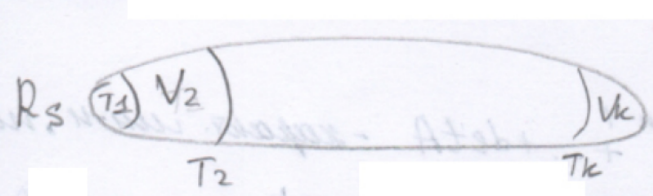
\includegraphics[width=0.5\linewidth]{"images/Issue7-1.png"}
  \caption[]{}
\end{figure}

\begin{theorem}
  Пусть $i > j$, тогда $\forall \overrightarrow{h}_i \in \mathcal{V}^i \, \exists \overrightarrow{h}_j \in \mathcal{V}^j: \overrightarrow{h}_j = B^{i-j}\overrightarrow{h}_i$.
\end{theorem}

\begin{proof}
  Построим такой $\overrightarrow{h}_j$ и покажем, что он лежит в $\mathcal{V}^j$.

  \[ B^j \overrightarrow{h}_j = B^j (B^{i-j}(h_i)) = (B^j B^{i-j} )(\overrightarrow{h}_i) = B^i \overrightarrow{h}_i = 0 \] 
  \[ B^{j-1} \overrightarrow{h}_j = B^{j-1} (B^{i-j}(h_i)) = (B^{j-1} B^{i-j} )(\overrightarrow{h}_i) = B^{i-1} \overrightarrow{h}_i \neq 0 \]
\end{proof}

Построение соответствующего базиса начинается с определения собственных векторов $A$, соответствующих числу $\overline{\lambda}$.
Для этого решается уравнение $(\overline{A} - \overline{\lambda} E) \overrightarrow{\overline{x}} = B  \overrightarrow{\overline{x}} = 0$.

Рассмотрим случай, когда имеется только один собственный вектор $\overrightarrow{e}$. В этом случае $k = l$ (наше подпространство будет представимо в виде 1 жордановой клетки). 
Вектор $\overrightarrow{e}$ образует базис в $\mathcal{V} = T_1$. Вектор $\overrightarrow{h}_1 \in \mathcal{V}^2$ найдём как решение $B \overrightarrow{h}_1 = \overrightarrow{e}$, по доказанной выше теореме такое уравнение имеет решение. 
Вектор $\overrightarrow{h}_1$ называется \textbf{присоединенным} к вектору $\overrightarrow{e}$. Вектора $\overrightarrow{e}$ и $\overrightarrow{h}_1$ образуют базис в $T_2$. 
Определим векторы $\overrightarrow{h}_i$, $i = \overline{2, l-1}$ из уравнений $B \overrightarrow{h_i} = \overrightarrow{h}_{i-1}$. Так построенные векторы $\overrightarrow{e}, \overrightarrow{h}_1, ..., \overrightarrow{h}_{l-1}$ образует базис в $R_s$. 
Этот базис называется жордановой цепью.

Запишем матрицу системы в этом базисе. Все построенные векторы находим из уравнений: 
$\overline{A}\overrightarrow{e} = \overline{\lambda} \overrightarrow{e}$, $\overline{A} \overrightarrow{h}_1 = \overrightarrow{e} + \overline{\lambda} \overrightarrow{h}_1$, ..., $\overrightarrow{A} \overrightarrow{h}_{l-1} = \overrightarrow{h}_{l-2} + \overline{\lambda} \overrightarrow{h}_{l-1}$

\[ \overline{A} = \begin{Vmatrix*} \overline{\lambda} & 1 & 0 & \cdots & \cdots \\
                              0 & \overline{\lambda} & 1 & 0 & \cdots     \\
                              \cdots & \cdots & \ddots & \cdots & \cdots \\
                              \cdots & \cdots & \cdots & \overline{\lambda} & 1 \\ 
                              \cdots & \cdots & \cdots & 0 & \overline{\lambda} 
             \end{Vmatrix*} \text{ -- жорданова клетка размер $l$}
             \]

В таком базисе системе имеет вид:

\begin{equation}
 \begin{cases}
   \cfrac{d \overline{x}^{\,1}}{dt} = \overline{\lambda} \overline{x}^{\,1} + \overline{x}^{\,2} \\
   \ldots \\
   \cfrac{d \overline{x}^{\,n-1}}{dt} = \overline{\lambda} \overline{x}^{\,n-1} + \overline{x}^{\,n} \\
   \cfrac{d \overline{x}^{\,n}}{dt} = \overline{\lambda} \overline{x}^{\,n} \\
 \end{cases} 
\end{equation}

Замена: $\overline{x}^{\,i} = \overline{y}^{\,i} e^{\overline{\lambda} t}$, $i = \overline{1, l} \Rightarrow \dot{\overrightarrow{y}}^{\,i} e^{\overline{\lambda} t} + \overline{\lambda} \dot{\overrightarrow{y}}^{\,i} e^{\overline{\lambda} t} = \lambda \dot{\overrightarrow{y}}^{\,i} e^{\overline{\lambda} t} + \dot{\overrightarrow{y}}^{\,i+1} e^{\overline{\lambda} t} \Rightarrow$
Система преобразуется к виду:

\begin{equation}
  \begin{cases}
    \cfrac{d\overline{y}^{\,1}}{dt} = \overline{y}^{\,2} \\ 
    \cfrac{d\overline{y}^{\,2}}{dt} = \overline{y}^{\,3} \\
    \ldots \\
    \cfrac{d\overline{y}^{\,l-1}}{dt} = \overline{y}^{\,l} \\
    \cfrac{d\overline{y}^{\,l}}{dt} = 0
  \end{cases}
  \Rightarrow 
  \overrightarrow{y} = \begin{Vmatrix*} C_l \cfrac{t^{l-1}}{(l-1)!} + C_{l-1} \cfrac{t^{l-2}}{(l-2)!} + ... + C_2 \cfrac{t}{1!} + C_1 \\
                            \ldots \\
                            \ldots \\
                            C_l t + C_{l-1} \\
                            C_l \end{Vmatrix*} \Rightarrow  
\end{equation}

\begin{equation*}
  \Rightarrow \overrightarrow{\overline{x}} = \begin{Vmatrix*} C_l \cfrac{t^{l-1}}{(l-1)!} + C_{l-1} \cfrac{t^{l-2}}{(l-2)!} + ... + C_2 \cfrac{t}{1!} + C_1 \\
    \ldots \\
    \ldots \\
    C_l t + C_{l-1} \\
    C_l \end{Vmatrix*} \cdot e^{\overline{\lambda} t} 
\end{equation*}


Переходим к старому базису: 

\[ \overrightarrow{x}(t) = \begin{Vmatrix*}
  \overrightarrow{e}, \overrightarrow{h}_1, ..., \overrightarrow{h}_{l-1} 
\end{Vmatrix*} \cdot \begin{Vmatrix*} C_l \cfrac{t^{l-1}}{(l-1)!} + C_{l-1} \cfrac{t^{l-2}}{(l-2)!} + ... + C_2 \cfrac{t}{1!} + C_1 \\
\ldots \\
\ldots \\
C_l t + C_{l-1} \\
C_l \end{Vmatrix*} \cdot e^{\overline{\lambda} t} \Rightarrow \] 

\begin{multline}
 \overrightarrow{x}^{\text{ об}}_0 =  \overrightarrow{e} \left(C_1 + ... + C_l \cfrac{t^{l-1}}{(l-1)!} \right) e^{\overline{\lambda} t} + ... + \overrightarrow{h}_{l-1} C_l e^{\overline{\lambda} t} = \\ 
  = \boxed{C_1 \overrightarrow{e} e^{\overline{\lambda} t} + C_2 (\overrightarrow{e} t + \overrightarrow{h}_1) e^{\overline{\lambda} t} + ... + C_l \left[ \overrightarrow{e} \cfrac{t^{l-1}}{(l-1)!} + \overrightarrow{h}_1 \cfrac{t^{l-2}}{(l-2)!} + ... + \overrightarrow{h}_{l-1} \right]} 
\end{multline}

Полагая последовательно $C_1 = 1, C_2 = ... = C_n = 0$; ...; $C_1 = ... = C_{i-1} = C_{i+1} = ... = C_n = 0$, $C_i = 1$, $i = \overline{2, n}$, получим функции:

$\overrightarrow{\varphi}_1 = \overrightarrow{e} e^{\overline{\lambda} t}$, $\overrightarrow{\varphi}_1 = (\overrightarrow{e}t + \overrightarrow{h}_1) e^{\overline{\lambda} t}$, ..., $\overrightarrow{\varphi}_{l-1} = \left(\overrightarrow{e} \cfrac{t^{l-1}}{(l-1)!} + \overrightarrow{h}_1 \cfrac{t^{l-2}}{(l-2)!} + ... + \overrightarrow{h}_{l-1}\right) e^{\overline{\lambda} t}$. 
Они являются решениями по построению, $W(0) = \begin{vmatrix*} ||\overrightarrow{e}, ..., \overrightarrow{h}_{l-1} ||\end{vmatrix*} \neq 0 \Rightarrow \overrightarrow{\varphi}_1, ..., \overrightarrow{\varphi}_{l-1}$ -- линейно независимы $\Rightarrow \overrightarrow{\varphi}_1, ..., \overrightarrow{\varphi}_{l-1}$ -- ФСР. 

\subsection{Линейная неоднородная система уравнений в случае, когда неоднородность представлена векторным квазимногочленом (без доказательства)}

\textbf{Источник: Романко В.К. Курс дифференциальных уравнений и вариационного исчисления}

\begin{definition}
  \textbf{Вектор-квазимногочленом} называется вектор-функция $\overrightarrow{f}(t) = e^{\mu t} \overrightarrow{P_m}(t)$, где $\mu$ -- заданное комплексное число, $\overrightarrow{P_m(t)}$ -- вектор-многочлен степени $m$, коэффициентами которого служат $n$-мерные векторы. 
\end{definition}

\begin{theorem}
  Если в системе $\dot{\overrightarrow{x}}(t) = A \overrightarrow{x}(t) + \overrightarrow{f}(t)$ $f(t) = e^{\mu t} \overrightarrow{P_m}(t)$, где $\overrightarrow{P_m}(t)$ -- вектор-многочлен степени $m$, тогда для этой системы всегда существует решение вида
  \[ \overrightarrow{x}(t) = e^{\mu t} \overrightarrow{Q_{m+k}}(t),\]
  где $\overrightarrow{Q_{m+k}}$ -- вектор-многочлен степени $(m + k)$, причём $k = 0$, если $\mu$ -- не собственное значение $A$, и $k$ не превосходит наибольшей длины жордановой цепочки для $\mu$, если $\mu$ -- собственное значние $A$, а коэффициентами $\overrightarrow{Q_{m+k}}(t)$ служат $n$-мерные числовые вектора.
\end{theorem}
